\chapter{Lösungsdesign}

Das Lösungsdesign beinhaltet die Grundlagen für die erfolgreiche Umsetzung des Prototypen. Dieses Kapitel beinhaltet die definierten Schnittstellen sowohl die Auswahl des Frameworks für die Darstellung. Ein besonderes Augenmerk wird auf die Interaktion zwischen der Visualisierung und dem \textit{ikc-core} gelegt, besonders auf die reduktion der Kopplung zwischen den beiden Komponenten. 

\section{Technische Ausgangslage}
Der \textit{ikc-core} funktioniert momentan mit einer puristischen Benutzeroberfläche. Die Applikationslogik und der Umgang mit der Datenbasis existieren somit bereits. Wie auf dem Komponentendiagramm (\autoref{fig:komponentendiagramm}) ersichtlich, nutzt der \textit{ikc-core} die Visualisierung (graph-visualization). Jedoch müssen dazu verschieden Schnittstellen auf der Visualisierung implementiert werden. Diese werden dann von der Visualisierung genutzt um Operation an den \textit{ikc-core} zu delegieren. Dies kann als Nutzungsvertrag zwischen der Visualisierung und dem Komponente, welche sie verwendet verstanden werden. Als Beispiel küm\-mert es die Visualisierung wenig, wie und wo ein Node gespeichert wird. Es wird nur die jeweilige Methode ausgeführt und alles andere geschieht ausserhalb der Vi\-su\-ali\-si\-erung. Mehr Details sind im \autoref{sec:architektur} zu finden.

\begin{figure}[htbp]
\centering
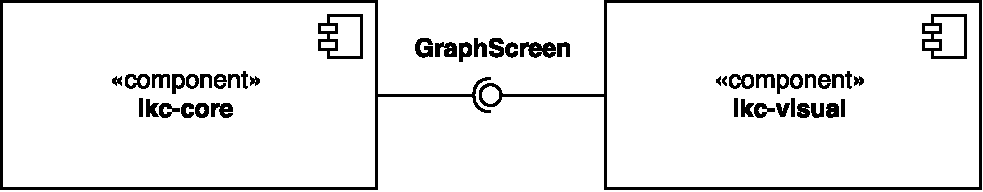
\includegraphics[width=0.6\textwidth]{components}
\caption{Komponentendiagramm}
\label{fig:komponentendiagramm}
\end{figure}

\section{Architektur}
\label{sec:architektur}

Das Klassendiagramm (\autoref{fig:klassendiagramm}) gewährt einen detaillierteren Überblick über die Architektur der Visualisierung. Es zeigt die Schnittstellen zum \textit{ikc-core} und die wichtigsten Komponenten auf.

\todo[inline]{Mehr Details?}

\begin{landscape}
\todo[inline]{Diagramm neuzeichnen (vektorisiert) und updaten (Signaturen)}

\begin{figure}[htbp]
\centering
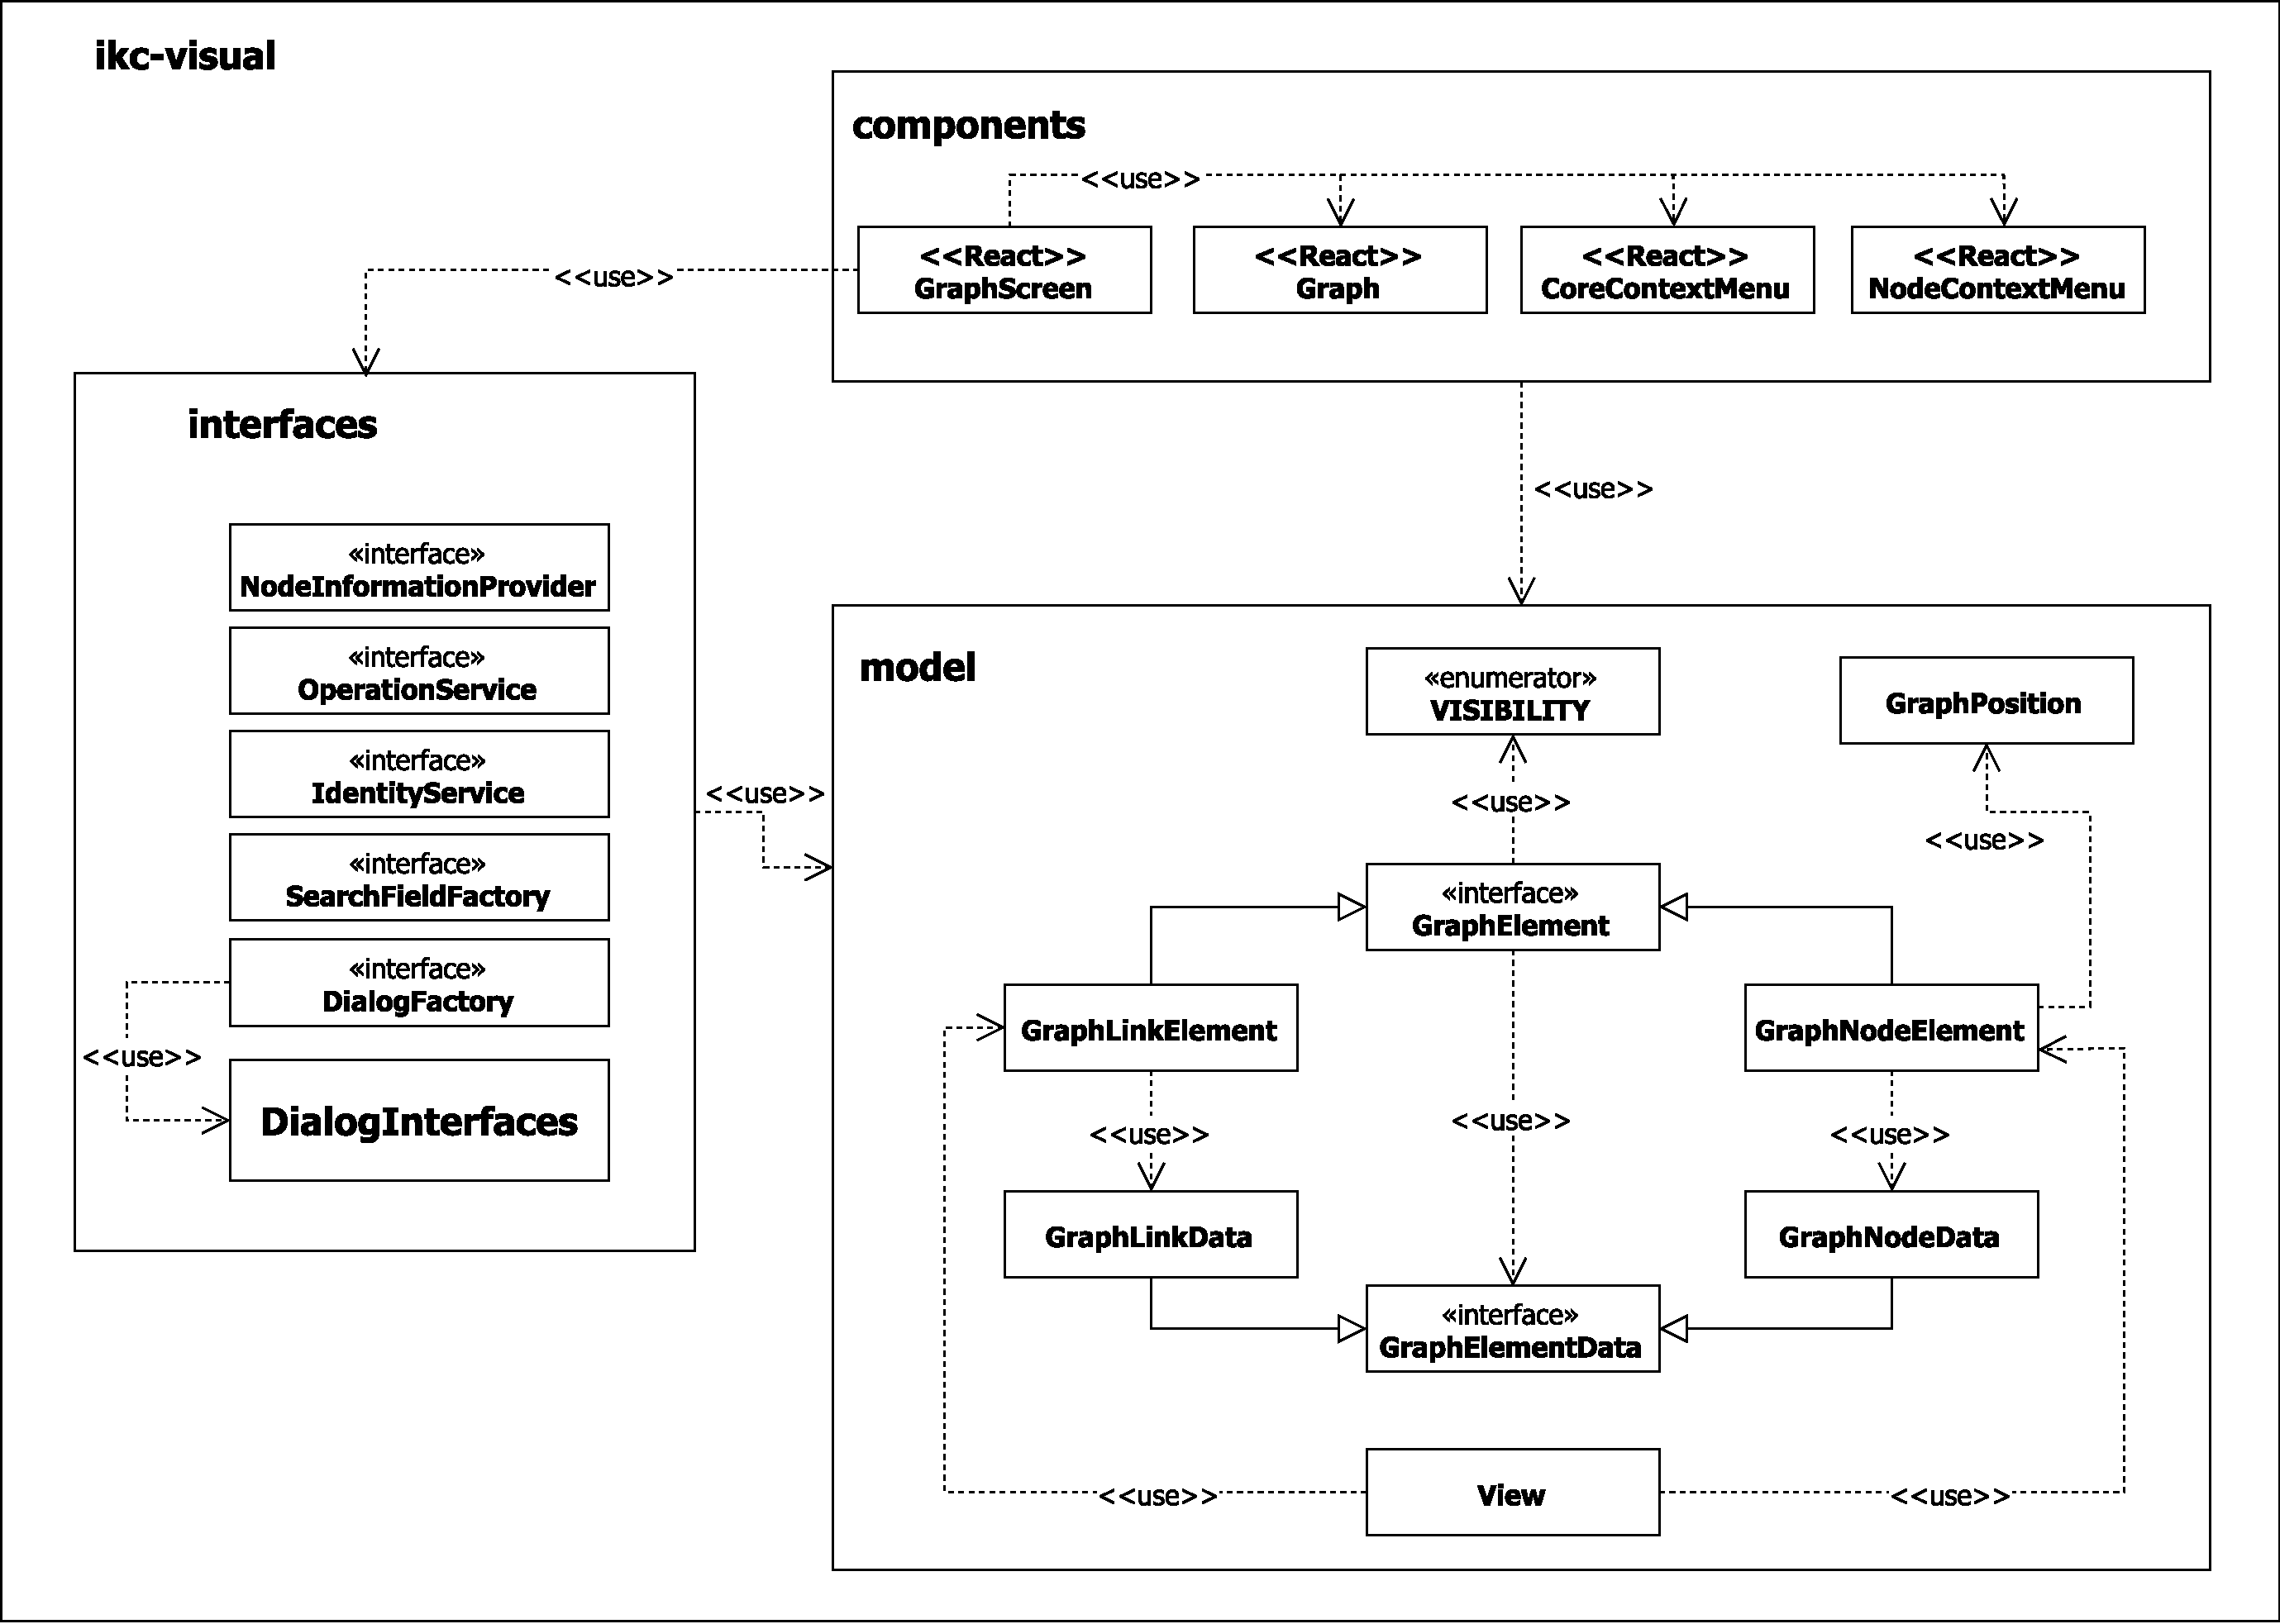
\includegraphics[width=1.6\textwidth]{architecture-overview}
\caption{Klassendiagramm}
\label{fig:klassendiagramm}
\end{figure}
\end{landscape}


\section{Schnittstellen} \label{schnittstellen}

Die hier gezeigten Schnittstellen dienen dem Austausch und der Interaktion mit dem \textit{ikc-core}. Um die Visualisierung in einer bestehenden Umgebung verwenden zu können, müssen die erforderlichen Teile implementiert werden.

Die \autoref{fig:integration-ikc-core} zeigt einen Teil einer möglichen Integration, beispielsweise in den bestehenden \textit{ikc-core}. Die rechte Seite stellt einen Ausschnitt des \textit{ikc-visual}-Paketes an. Die Klasse \textit{GraphScreen} (\autoref{GraphScreen}) ist zu\-stä\-ndig für die Visualisierung des Netzwerkes. Um den vollen Funktionsumfang zu bieten, benutzt sie, unter anderem, die Schnittstelle \textit{DialogFactory} (!!!REFERENZ!!!). Diese soll den Umgang mit Dialogfenstern ermöglichen. Da dies zu den grundlegenden Funktionen der Visualisierung zählt, befindet sich diese Schnittstelle direkt im \textit{ikc-visual}-Paket. Bei der Integration der Visualisierung in eine bestehende Umgebung gilt es somit, die verschiedenen Schnittstellen entsprechend zu implementieren.

Die Klasse \textit{GraphVisualisation} verwendet die Klasse \textit{GraphScreen} aus der Visualisierung. Folglich muss beispielsweise die Schnittstelle \textit{DialogFactory} implementiert werden. Dies wird mit der Klasse \textit{GraphDialogFactory} realisiert.

Ähnlich wie beim oben beschriebenen Beispiel gibt es weitere Voraussetzungen des \textit{GraphScreen}, welche bei einer Integration beachtet werden sollten. Diese werden nachfolgenden genau erläutert.

\todo[inline]{Referenzen zu folgenden Unterkapiteln}

Es folgt eine Beschreibung der im \textit{ikc-visual}-Paket enthaltenen Klassen und Schnittstellen. 
\begin{figure}[htbp]
\centering
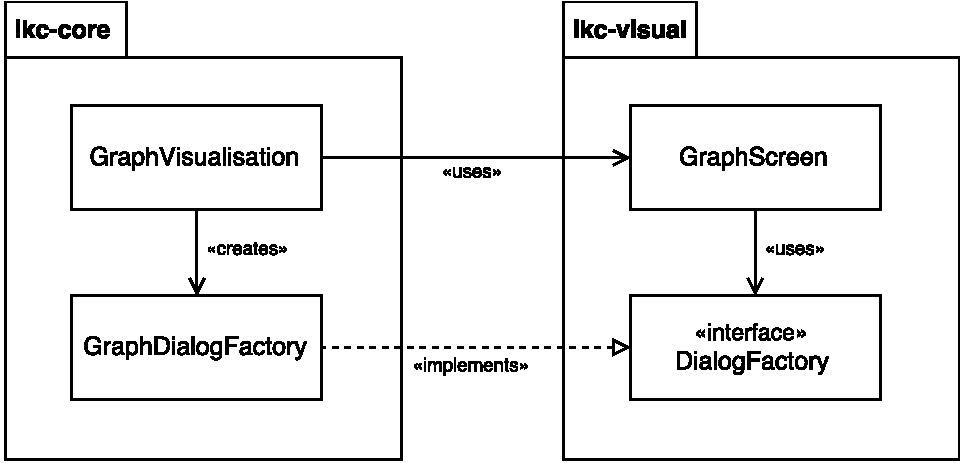
\includegraphics[width=0.7\textwidth]{architecture}
\caption{Integration ikc-core}
\label{fig:integration-ikc-core}
\end{figure}

\subsection{NodeComponentFactory}
Mit dem \textit{Factory-Pattern} wird die Objekterzeugung von der tatsächlichen Implementation entkoppelt. Dies wird verwendet um die Komponentenrepräsentationen der Knoten und Kanten auszuliefern (\autoref{lst:nodecomponentfactory}).

\begin{listing}[htbp]
\inputminted[
frame=lines,
framesep=2mm,
baselinestretch=1.2,
linenos,
breaklines=true
]{js}{sourcecode/common/interfaces/NodeComponentFactory.ts}
\caption{NodeComponentFactory-Interface}
\label{lst:nodecomponentfactory}
\end{listing}

\subsection{NodeInformationProvider}
Die Visualisierung benötigt zum Darstellen des Netzwerk diverse Informationen zu den einzelnen Knoten und Kanten. Diese werden über die beiden Methoden \texttt{getNodeTitle} und \texttt{getNodeEdgesIds} geliefert. Die Identifikation erfolgt jeweils über eine eindeutige Identifikationsnummmer (\autoref{listing:nodeinformationprovider}).

Teile der Visualisierung sollen mittels \textit{Drag and Drop} bedient werden können. Folgend ein Beispiel, wie die Schnittstelle in diesem Anwendungsfall benutzt werden kann:

Beim \textit{Drag and Drop} wird üblicherweise ein \textit{Event} beim Loslassen des gepackten Elements ausgelöst. Das Element soll eine eindeutige Identifikationsnummer (ID) enthalten. Dies ist aus dem bestehenden \textit{IKC-Core} vorausgesetzt. Wird das Element nun innerhalb der Visualisierung losgelassen, enthält der ausgelöste \textit{Event} so auch diese ID. Diese kann zusammen mit dem \textit{Event} abgefangen und wiederverwendet werden. Beispielsweise können nun Informationen über den \textit{NodeInformationProvider} bezogen werden.

\begin{listing}[htbp]
\inputminted[
frame=lines,
framesep=2mm,
baselinestretch=1.2,
linenos,
breaklines=true
]{js}{sourcecode/common/interfaces/NodeInformationProvider.ts}
\caption{NodeInformationProvider-Interface}
\label{listing:nodeinformationprovider}
\end{listing}

\subsection{OperationService}
Die \textit{OperationService}-Schnittstelle ermöglicht der Visualisierung mit der Datenbasis zu interagieren. Wird beispielsweise in der Visualisierung ein neuer Knoten erstellt, muss dieser auch auf der Datenbasis erzeugt werden (\autoref{listing:operationservice}). 

Lesezugriffe erfolgen aber über den zuvor genannten \textit{NodeInformationProvider} (\autoref{listing:nodeinformationprovider}).

\begin{listing}[htbp]
\inputminted[
frame=lines,
framesep=2mm,
baselinestretch=1.2,
linenos,
breaklines=true
]{js}{sourcecode/common/interfaces/OperationService.ts}
\caption{OperationService-Interface}
\label{listing:operationservice}
\end{listing}

\subsection{View}
Die \textit{View} ist eine Abstraktion der Visualisierung. Sie hält einerseits Informationen zu der einzelnen Sicht, welche Kanten und Knoten sind sichtbar. Andererseits ermöglichst sie auch das persistieren der Sicht. Dies erfolgt über eine \textit{JSON}-Repräsentation (\autoref{listing:view}).

\begin{listing}[htbp]
\inputminted[
frame=lines,
framesep=2mm,
baselinestretch=1.2,
linenos,
breaklines=true
]{js}{sourcecode/common/interfaces/View.ts}
\caption{View-Interface}
\label{listing:view}
\end{listing}

\section{Komponenten}\label{komponenten}

Die \textit{React}-Komponenten werden seitens der Visualisierung implementiert. Der \textit{Graphscreen} (\autoref{listing:graphscreen}) beinhaltet hier \textit{DiagramNodes} (\autoref{listing:diagramnode}) und \textit{DiagramEdges} (\autoref{listing:diagramedge}). Für die grafische Repräsentation der verschiedenen Komponenten werden direkt \textit{React}-Komponenten verwendet (vgl. \autoref{sec:technologie}).

\subsection{DiagramEdge}
Eine Kante wird mithilfe der Komponente \textit{DiagramEdge} dargestellt. Diese hat Eigenschaften wie 

\begin{itemize}
  \setlength\itemsep{1em}
    \item \textbf{label}: Allfällige Beschriftung der Kante (Links).
    \item \textbf{sourceNodeId}: ID des Ursprungsknotens.
    \item \textbf{destNodeId}: ID des Zielknotens.
    \item \textbf{direction}: Richtung des Links.
\end{itemize}

, welche die Kante näher beschreiben (\autoref{listing:diagramedge}). Die Richtung des \textit{Links} ergibt sich aus der Angabe von \textit{Source-} und \textit{DestinationNodeId}.

\begin{listing}[H]
\inputminted[
frame=lines,
framesep=2mm,
baselinestretch=1.2,
linenos,
breaklines=true
]{js}{sourcecode/common/components/DiagramEdgeInterface.tsx}
\caption{DiamgramEdge-Komponente}
\label{listing:diagramedge}
\end{listing}

\subsection{DiagramNode}
Ähnlich wie die \textit{DiagramEdge} funktioniert die Repräsentation auch bei der \textit{DiagramNode}. Wiederum sind hier Eigenschaften vorgegeben, welche zusätzlich Informationen zum Knoten beinhalten (\autoref{listing:diagramnode}):

\begin{itemize}
    \item \textit{id}: ID
    \item \textit{label}: Beschriftung
    \item \textit{positionX}, \textit{positionY}: Koordinaten
    \item \textit{detailComponenten}: Kind-Komponente für weitere Informationen
\end{itemize}

\begin{listing}[htbp]
\inputminted[
frame=lines,
framesep=2mm,
baselinestretch=1.2,
linenos,
breaklines=true
]{js}{sourcecode/common/components/DiagramNodeInterface.tsx}
\caption{DiamgramNode-Komponente}
\label{listing:diagramnode}
\end{listing}

\subsection{GraphScreen}\label{GraphScreen}
Die \textit{GraphScreen}-Komponente sammelt alle Abhängigkeiten und repräsentiert das Netzwerk als Ganzes. Sie hält alle Referenzen zu Daten, Funktionen sowie zu den umliegenden Komponenten und bildet damit ein wichtiges Bindeglied zwischen \textit{ikc-core} und der Visualisierung. Nachfolgend weitere Informationen zu den Eigenschaften (\autoref{listing:graphscreen}):

\begin{itemize}
    \item \textit{viewToLoad}: Sicht, welche angezeigt wird.
    \item \textit{onViewSave}: Funktion, welche zum Speichern der Sicht aufgerufen wird.
    \item \textit{onViewDelete}: Funktion, welche zum Löschen der Sicht aufgerufen wird.
    \item \textit{nodeComponentFactory}: \textit{Factory}, welche Knoten und Kanten liefert.
    \item \textit{nodeInformationProvider}: Stellt Informationen zu Knoten und Kanten zur Verfügung.
    \item \textit{operationService}: Ermöglicht Interkation mit Datenbasis.
\end{itemize}

\begin{listing}[htbp]
\inputminted[
frame=lines,
framesep=2mm,
baselinestretch=1.2,
linenos,
breaklines=true
]{js}{sourcecode/common/components/GraphScreenInterface.tsx}
\caption{GraphScreen-Komponente}
\label{listing:graphscreen}
\end{listing}

In \autoref{listing:graphscreenexample} ist ein Beispiel für die Verwendung aufgezeigt. 

\begin{listing}[htbp]
\inputminted[
frame=lines,
framesep=2mm,
baselinestretch=1.2,
linenos,
breaklines=true
]{js}{sourcecode/GraphScreenExample.tsx}
\caption{GraphScreen-Beispiel}
\label{listing:graphscreenexample}
\end{listing}

\section{Framework-Auswahl}
Um sicherzustellen, dass ein geeignetes \textit{Framework} für die Visualisierung verwendet wird, müssen verschiedene Optionen untersucht und bewertet werden.
\subsection{Kriterien-Katalog}
Für die Bewertung wird ein Katalog an Kriterien definiert, welcher sich an den definierten Anforderungen (siehe \autoref{anforderungen}), Risikoanalyse (siehe \autoref{risikoanalyse}), Schnittstellen (siehe \autoref{schnittstellen}) und Komponenten (siehe \autoref{komponenten}) orientiert. Folgend eine Übersicht über den Kriterienkatalog (\autoref{tab:kriterien-katalog}). 

\begin{longtable}{|p{1cm}| p{3cm} | p{8.1cm}|}
  \hline
    ID & Titel &  Beschreibung \\\hline
    K1 & Mobile Darstellung & Das Framework kann im Mobile Umfeld verwendet werde\\\hline
    K2 & Operationen & Es können die folgenden Operationen umgesetzt werden:
        \begin{enumerate}
          \item Einen neuen Node innerhalb Visualisierung erstellen.
          \item Zwei Nodes innerhalb Visualisierung verbinden.
          \item Einen Node innerhalb der Visualisierung löschen.
        \end{enumerate} \\\hline
    K3 & Operationen (D'n'D\footnote{Drag and Drop}) & Es können die folgenden D'n'D-Operationen umgesetzt werden:
        \begin{enumerate}
          \item Einen neuen Node mittels Drag'n'Drop innerhalb der Visualisierung erstellen.
          \item Zwei Nodes innerhalb der Visualisierung mittels Drag'n'Drop verbinden.
        \end{enumerate} \\\hline
    K4 & Node Details & Node Details können angezeigt und bearbeitet werden.\\\hline
    K5 & Menu & Ein Kontextmenü für weitere Operationen anzeigen.\\\hline
    K6 & Nodes Speichern & Positionen der Nodes können gespeichert werden.\\\hline
    K7 & Nodes Laden & Eine bestehende View kann dargestellt werden.\\\hline
    K8 & Toolbox & Weitere Operationen, z.b. Suche, können in einer Toolbox angeboten werden.\\\hline
    K9 & Komplexität & Allgemeiner Eindruck des Frameworks hinsichtlich der Komplexität.\\\hline
    K10 & Erweiterbarkeit & Allgemeiner Eindruck des Frameworks hinsichtlich der Erweiterbarkeit.\\\hline
    K11 & Dokumentation & Das Framework ist gut dokumentiert, es gibt genügend Beispiele und eine entsprechende \textit{Community} zur allfälligen Unterstützung.\\\hline
    \caption{Kriterienkatalog}
  \label{tab:kriterien-katalog}
\end{longtable}
Mit Hilfe dieses Katalogs sollen die Möglichkeiten, Chancen und auch Risiken der verschiedenen \textit{Frameworks} identifiziert werden. Aufgrund dieses Prozesses kann anschliessend eine genaue Einschätzung der Möglichkeiten und des Aufwands aufgestellt werden. Die verschiedenen  \textit{Frameworks} werden anhand der folgenden Skala bewertet (1-5): 
\begin{enumerate}
  \item Die Erfüllung des Kriteriums ist mit diesem Framework ohne Anpassungen möglich.
  \item Die Erfüllung des Kriteriums ist mit diesem Framework mit leichten Anpassungen möglich.
  \item Die Erfüllung des Kriteriums ist mit diesem Framework mit Anpassungen möglich.
  \item Die Erfüllung des Kriteriums ist mit diesem Framework mit grossen Anpassungen möglich.
  \item Die Erfüllung des Kriteriums ist mit diesem Framework nicht möglich.
\end{enumerate}

\subsection{Ergebnisse}
Aufgrund des definierten Kriterienkataloges wurden die verschiedenen \textit{Frameworks} untersucht und bewertet. Die Ergebnisse sind in folgender \autoref{tab:framework-auswertung} aufgeführt. Die Tabelle widerspiegelt die Eindrücke und Erfahrungen, welche während den Untersuchen gemacht wurden:

Zwar sind auch die umfassenderen Lösungen sehr interessant, jedoch ist deren Verwendung für den hier notwendigen Zweck zu kompliziert. Es würde lediglich ein kleiner Teilbereich der bereits bestehenden Lösung genutzt. Um aber diesen erfolgreich einzusetzen, ist dennoch tiefe Kenntnis des jeweiligen \textit{Frameworks} erforderlich. Dies sprengt schlichtweg den zeitlichen Rahmen und ist auch nicht notwendig. Die nötigen Erweiterungen können in den anderen, schlankeren \textit{Frameworks} ohne grossen Zusatzaufwand ergänzt werden.

Darum fiel die Wahl eindeutig auf \textit{cytoscape.js}. Es beschränkt sich lediglich auf die Darstellung von Netzwerken. Erweiterungen sind bereits diverse zugänglich. Auch ist es gleichzeitig relativ einfach den Funktionsumfang eigenhändig zu ergänzen.

\begin{longtable}{|p{0.8cm}| p{2.2cm} | p{1.5cm}| p{1.5cm}| p{2cm}| p{2cm}|}
  \hline
    & \textit{cytoscape.js} & \textit{greuler} &\textit{JointJS} &\textit{jsPlumb} &\textit{mxGraph}  \\\hline
    Total & 23 & 27 & 38 & &\\\hline
    \caption{Framework-Auswerung}
  \label{tab:framework-auswertung}
\end{longtable}

\subsection{Bewertungen}\label{Bewertungen}
Eine detaillierte Bewertung der fünf verschiedenen \textit{Frameworks} kann den folgenden Abschnitten entnommen werden.

\subsubsection{cytoscape.js}
\label{cytoscape}
Cytoscape ist eine \textit{open-source} Javascript Bibliothek für Graphen- oder Netzwerk-Theorie. Sie eignet sich nicht nur für Visualisierungen, sondern auch für Analysen. Cytoscape ist mit allen gängigen Browsern und Bibliotheken kompatibel. Auch funktioniert die Darstellung ohne zusätzlichen Aufwand auf allen Bildschirmgrössen. Es gibt zahlreiche Erweiterungen und auch die Integration in bestehende Lösungen ist einfach möglich. \cite{1_franz_lopes_huck_dong_sumer_bader_2016}

Wie in \autoref{fig:bsp-cytoscape} ersichtlich, beschränkt sich die Bibliothek lediglich auf die Visulisierung von Netzwerken. Standardmässig sind keine Zusatzfunktionen, beispielsweise das Interagieren mit \textit{Nodes} und \textit{Links} möglich. Im Gegenzug ist die Bibliothek sehr schlank gehalten, was eine einfache Integration und Erweiterung stark vereinfacht. Das Netzwerk wird direkt im \textit{JSON}-Format hinterlegt. Sollen Änderungen vorgenommen werde, werden die hinterlegten Daten angepasst und anschliessend angezeigt.

\begin{figure}[htbp]
\centering
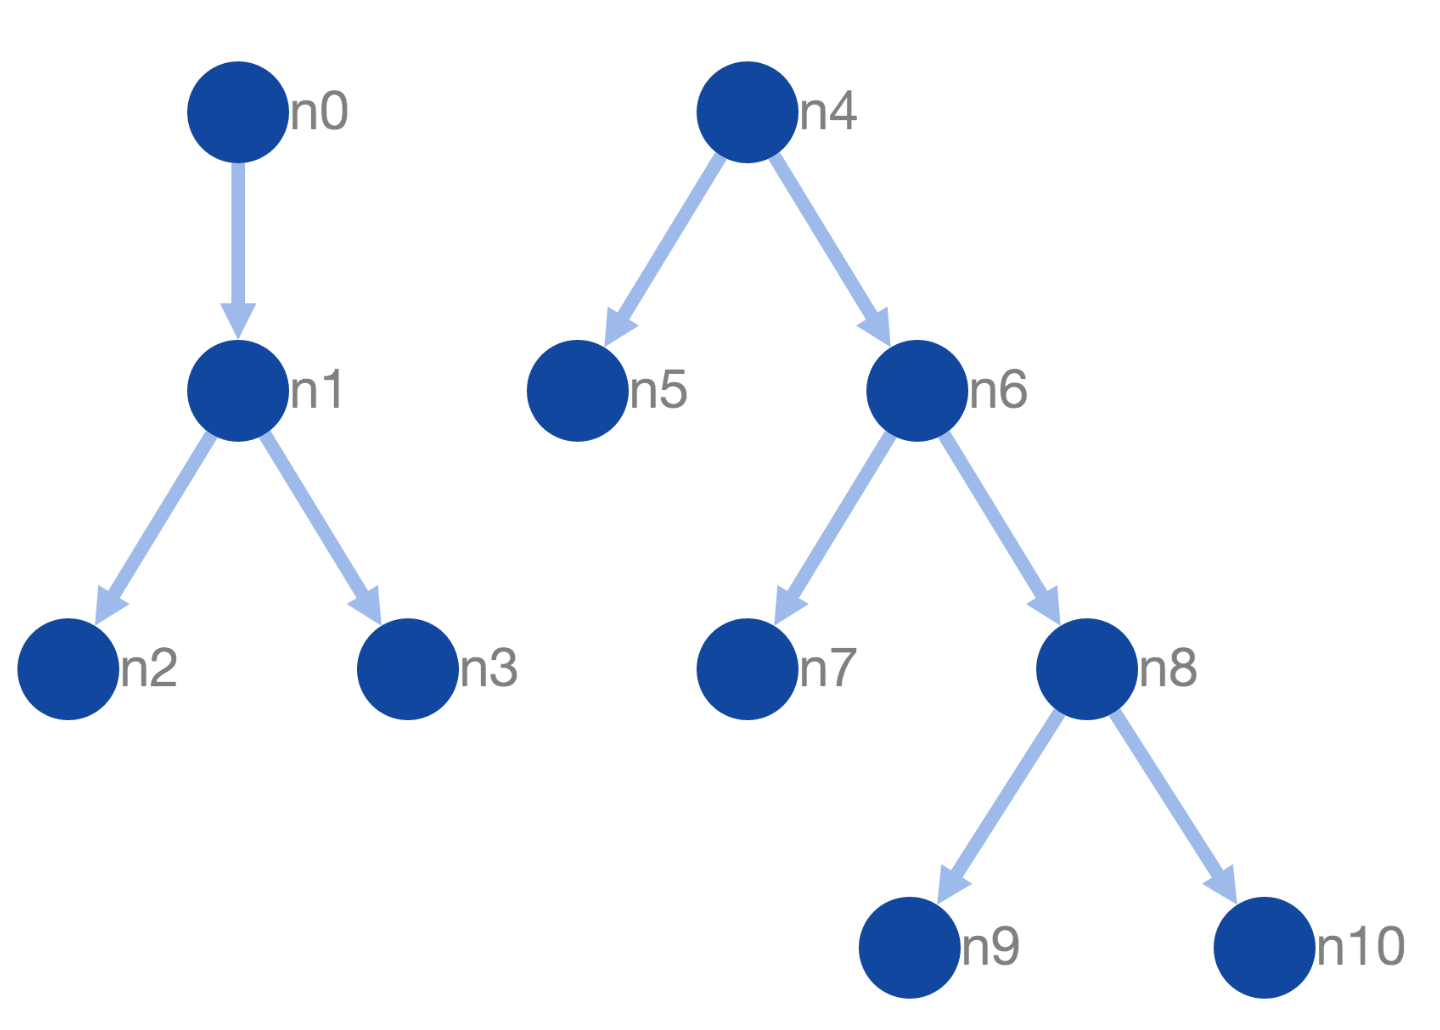
\includegraphics[width=0.4\textwidth]{cytoscape}
\caption{Beispiel Cytoscape}
\label{fig:bsp-cytoscape}
\end{figure}


\begin{longtable}{|p{0.5cm}|p{0.5cm}|p{0.5cm}|p{0.5cm}|p{0.5cm}|p{0.5cm}|p{0.5cm}|p{0.5cm}|p{0.5cm}|p{0.7cm}|p{0.7cm}|}
  \hline
    K1 & K2 & K3 & K4 & K5 & K6 & K7 & K8 & K9 & K10 & K11 \\\hline
    2 & 2 & 2 & 2 & 2 & 2 & 3 & 2 & 2 & 3 & 1\\\hline
    \caption{Bewertung  \textit{cytoscape.js}}
  \label{tab:bewertung-cytoscape}
\end{longtable}

\subsubsection{greuler}
Hier gibt es viele Parallen zur vorgängigen Bibliothek (\autoref{cytoscape}). \textit{Greuler} spezialisert sich nun aber auf die Visualisierung, baut wie viele andere auf \textit{D3}. Bezüglich der Handhabung ist es grösstenteils identisch mit \textit{Cytoscape}, allerdings hat hier es bei weiten nicht so viele Erweiterungsmöglichkeiten. \autoref{fig:bsp-greuler} zeigt ein kleines Beispielnetzwerk. \cite{2_maurizzzio/greuler_2016}

\begin{figure}[htbp]
\centering
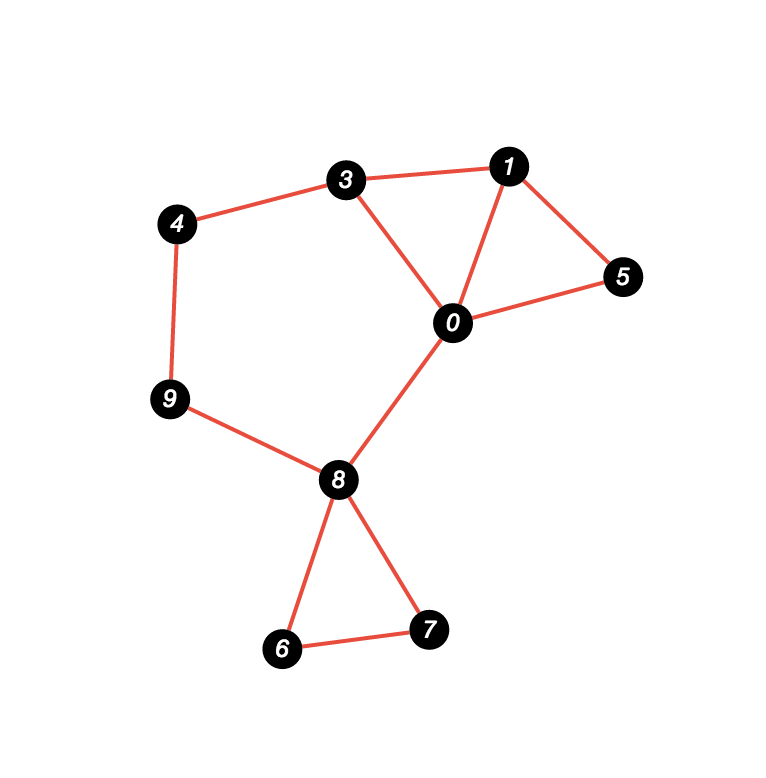
\includegraphics[width=0.4\textwidth]{greuler}
\caption{Beispiel Greuler}
\label{fig:bsp-greuler}
\end{figure}

\begin{longtable}{|p{0.5cm}|p{0.5cm}|p{0.5cm}|p{0.5cm}|p{0.5cm}|p{0.5cm}|p{0.5cm}|p{0.5cm}|p{0.5cm}|p{0.7cm}|p{0.7cm}|}
  \hline
    K1 & K2 & K3 & K4 & K5 & K6 & K7 & K8 & K9 & K10 & K11 \\\hline
    2 & 2 & 2 & 2 & 2 & 4 & 4 & 2 & 2 & 4 & 3\\\hline
    \caption{Bewertung \textit{greuler}}
  \label{tab:bewertung-greuler}
\end{longtable}

\subsubsection{JointJS}
Auch bei JointsJS handelt es sich um eine \textit{open-source}-Bibliothek. Im Gegensatz zu den obigen beiden geht die Funktionalität einen Ebene weiter. Hier werden zusätzlich zur eigentlichen Darstellung auch Werkzeuge zur Manipulation des Diagramms mitgeliefert. Viele Funktionalitäten sind aber erst mit der kostenpflichten Version \textit{Rappid} ver\-füg\-bar, welche auf JointJS aufbaut. \cite{jointsjs}

Die Bibliothek ist für den hier vorliegenden Anwendungsfall zu umfangreich. Die vielen Funktionen machen die Implementation sehr komplex. Dieser Aufwand ist für die eigentliche einfache Anwendung übertrieben. Die Vorteile, welche der vorhandene Funktionsumfang und auch wirklich genutzt werden, können vergleichsweise schnell selbst implementiert werden. So ist die Übersicht stets vorhanden.

\begin{longtable}{|p{0.5cm}|p{0.5cm}|p{0.5cm}|p{0.5cm}|p{0.5cm}|p{0.5cm}|p{0.5cm}|p{0.5cm}|p{0.5cm}|p{0.7cm}|p{0.7cm}|}
  \hline
    K1 & K2 & K3 & K4 & K5 & K6 & K7 & K8 & K9 & K10 & K11 \\\hline
    1 & 3 & 3 & 3 & 3 & 4 & 4 & 5 & 4 & 5 & 3\\\hline
    \caption{Bewertung \textit{JointJS}}
  \label{tab:bewertung-jointjs}
\end{longtable}

\subsubsection{jsPlumb}

\todo[]{Bewertung der Frameworks inkl. kleiner Text + Screenshoot}

\begin{longtable}{|p{0.5cm}|p{0.5cm}|p{0.5cm}|p{0.5cm}|p{0.5cm}|p{0.5cm}|p{0.5cm}|p{0.5cm}|p{0.5cm}|p{0.7cm}|p{0.7cm}|}
  \hline
    K1 & K2 & K3 & K4 & K5 & K6 & K7 & K8 & K9 & K10 & K11 \\\hline
    & & & & & & & & & &\\\hline
    \caption{Bewertung \textit{jsPlumb}}
  \label{tab:bewertung-jsplumb}
\end{longtable}


\subsubsection{mxGraph}

\begin{longtable}{|p{0.5cm}|p{0.5cm}|p{0.5cm}|p{0.5cm}|p{0.5cm}|p{0.5cm}|p{0.5cm}|p{0.5cm}|p{0.5cm}|p{0.7cm}|p{0.7cm}|}
  \hline
    K1 & K2 & K3 & K4 & K5 & K6 & K7 & K8 & K9 & K10 & K11 \\\hline
    & & & & & & & & & &\\\hline
    \caption{Bewertung \textit{mxGraph}}
  \label{tab:bewertung-mxgraph}
\end{longtable}

 
\section{User Interface Design}

Folgend werden wichtige Punkte zum Umgang mit dem Netzwerk und zur Integration der Visualisierung aufzeigt und weitergehende Überlegungen dazu dargelegt.

\subsection{Umgang mit dem Netzwerk}

Die Benutzeroberfläche orientiert sich hauptsächlich am Netzwerk bestehend aus Nodes und Links. Diese besitzen eine Beschriftung in Form des Titels, oder in Form des entsprechenden \textit{Tags} (\autoref{fig:nodes-links}). Diese können zugunsten der Übersichtlichkeit gegebenenfalls ausgeblendet werden.

Wo immer möglich soll die Interaktion nicht über eine entfernte Schaltfläche, sondern direkt am jeweiligen Element in der Visualisierung geschehen. Ein mögliches Beispiel dafür zeigt \autoref{fig:node-menu}. Gleich beim Knoten, wo eine Aktion vorgenommen werden soll, kann mittels eines Klicks (oder Ähnlichem) ein Kontextmenü geöffnet werden. Dies ermöglicht der Situation entsprechende, weiterführende Funktionalitöten. Entsprechende Möglichkeiten sind auch beim Umgang mit Kanten vorstellbar.

\begin{figure}[htbp]
\centering
 \begin{subfigure}{0.35\textwidth}
        \centering
        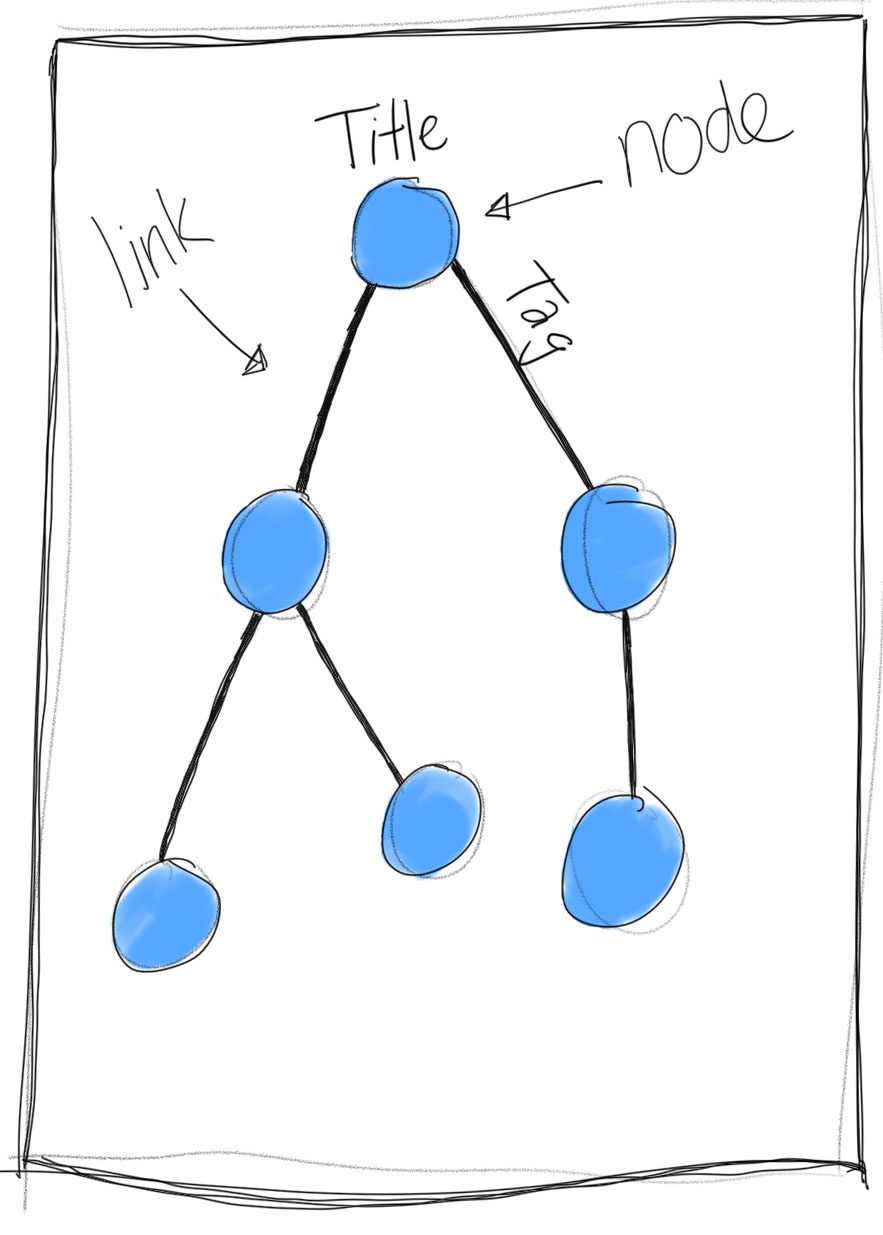
\includegraphics[width=0.9\linewidth]{skizze-nodes-links}
        \caption{Nodes und Links}
        \label{fig:nodes-links}
    \end{subfigure}
 \begin{subfigure}{0.35\textwidth}
        \centering
        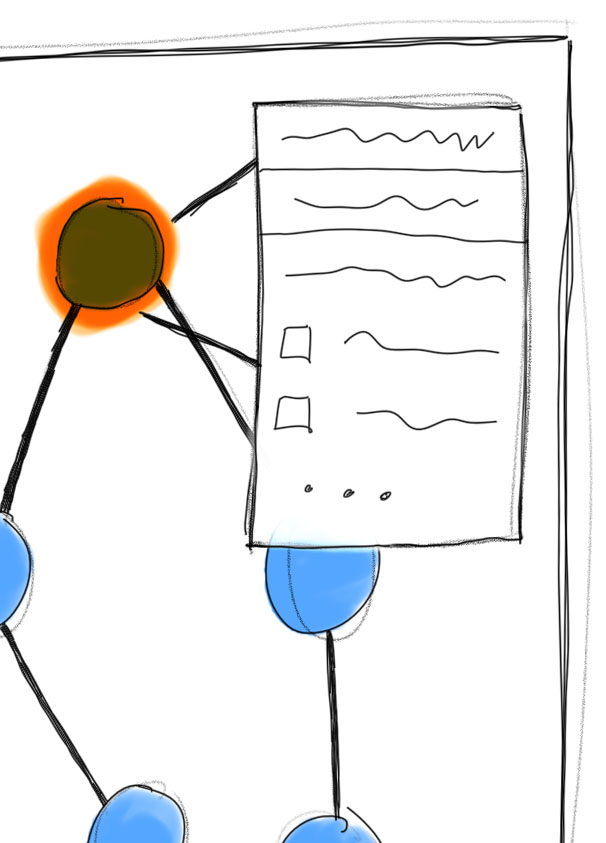
\includegraphics[width=0.9\linewidth]{skizze-contextmenu}
        \caption{Node-Menü}
        \label{fig:node-menu}
    \end{subfigure}
    \caption{Skizzen Benutzeroberfläche}
\end{figure}

\subsection{Integration}

Aus den Anforderungen geht die Interaktion mit dem \textit{ikc-core} als weiterer wichtiger Punkt hervor. Von besonderer Bedeutung ist hier die Bedienung mittels \textit{Drag and Drop}. Wie in \autoref{fig:grenze-core-visual} sichtbar, muss dabei die Grenze zwischen \textit{ikc-core} und der Visualisierung (grüne Linie) überwunden werden. Mittels \textit{Drag and Drop} kann also beispielweise ein Node aus der \textit{ikc-core}-Komponente (orange) in die Visualisierung positioniert werden. Dort kann dieser weiter mit dem bestehenden Netzwerk verknüpft oder als eigenständiger neuer Knoten dargestellt werden.

\begin{figure}[htbp]
\centering
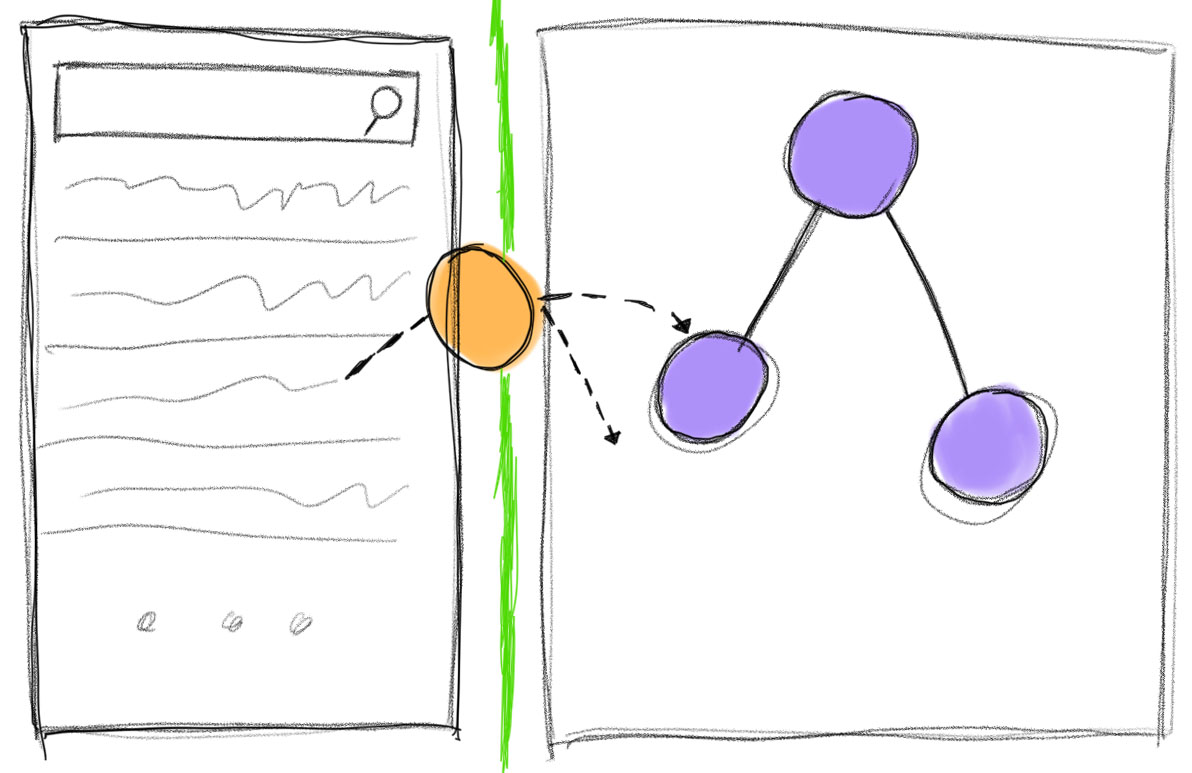
\includegraphics[width=0.5\textwidth]{ikc-core-visual}
\caption{Grenze ikc core - visual}
\label{fig:grenze-core-visual}
\end{figure}

Wo immer möglich sollen bestehende Komponenten wiederverwendet werden. Dies bietet sich nicht nur bei \autoref{fig:node-menu} in Form eines Kontextmenüs, sondern auch für die Suchfunktion und die Detailansicht an. Für die Desktop-Ansicht wird die Visualisierung mittig in einer dreispaltigen Anordnung in den \textit{ikc-core} eingebettet (\autoref{fig:3-column}). Auf der linken Seite befindet sich die Suche. Auf der rechten Seite die Detailansicht für den in der Visualisierung ausgewählten Node. Dort sind auch weitere Optionen beispielsweise in Form von Menüpunkten, den ausgehenden Link erreichbar. Zusätzlich gibt es eine übergeordnete Navigationsleiste, wo wichtige Funktion direkt abrufbar sind.

Bei der Version für Tablets und Smartphones sind, je nach verfügbarer Breite, nur eine oder zwei Spalten sichtbar.


\begin{figure}[htbp]
\centering
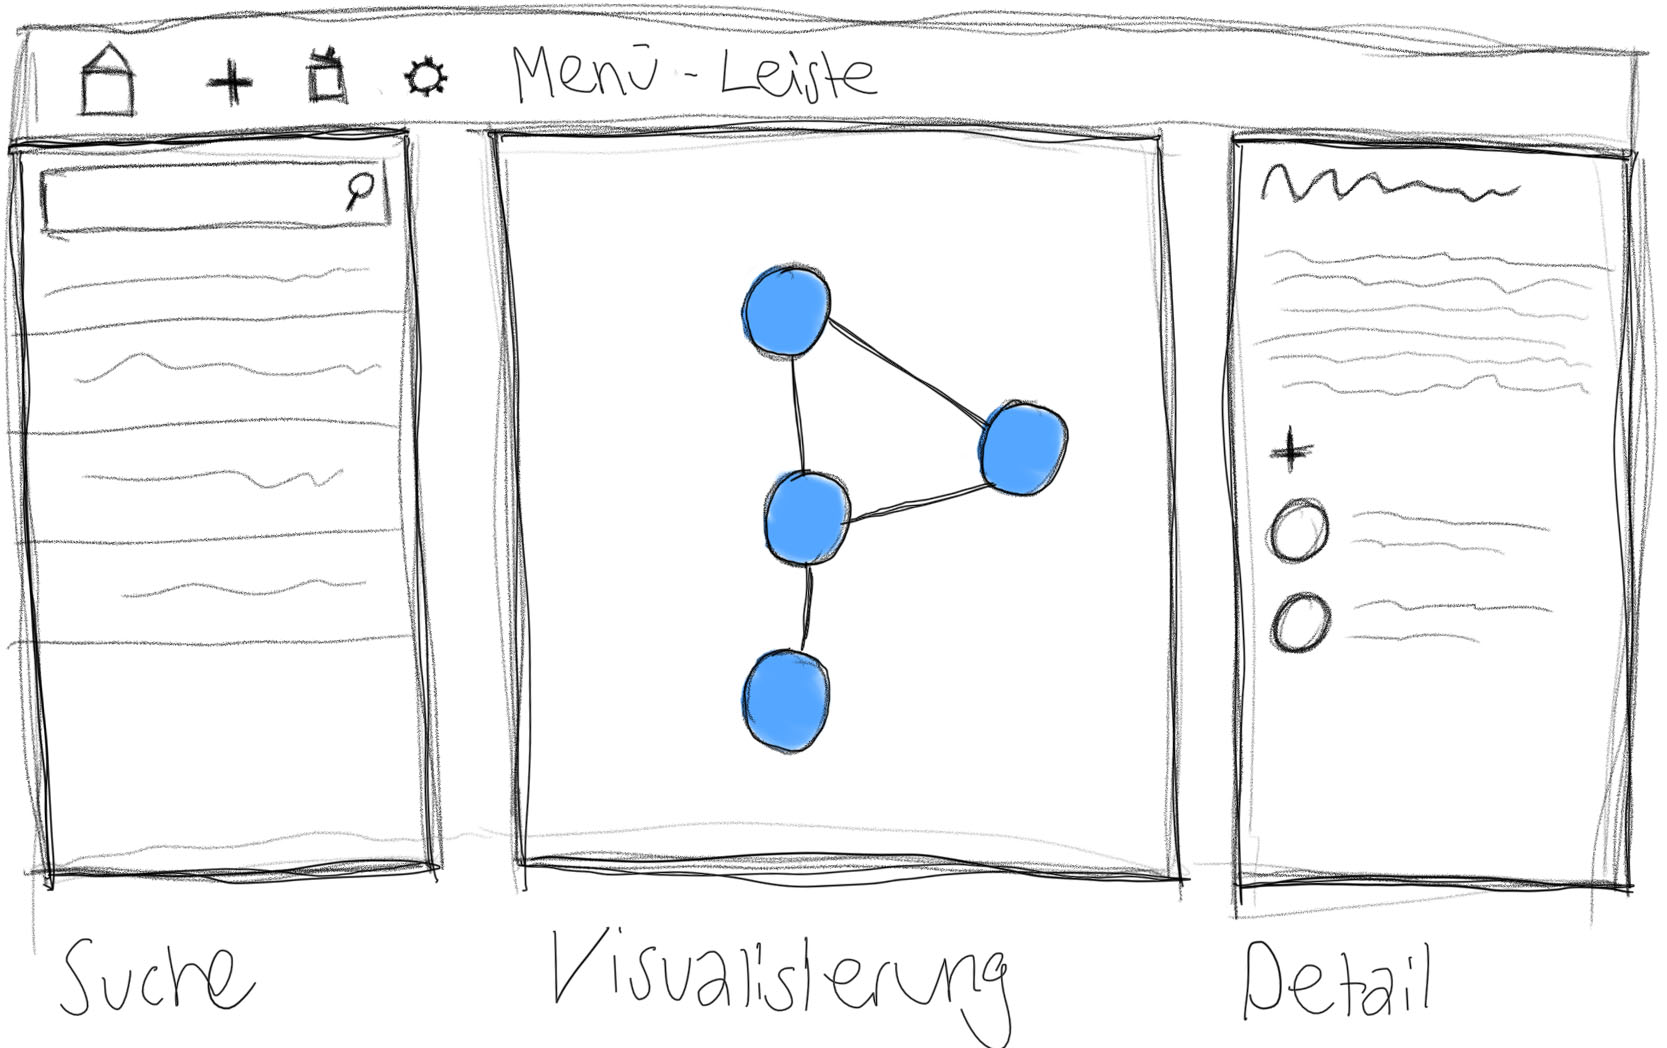
\includegraphics[width=0.8\textwidth]{integration-3-column}
\caption{3-spaltige Oberfläche}
\label{fig:3-column}
\end{figure}